\documentclass{article}
\usepackage{tikz}
\usetikzlibrary{arrows.meta}

\begin{document}

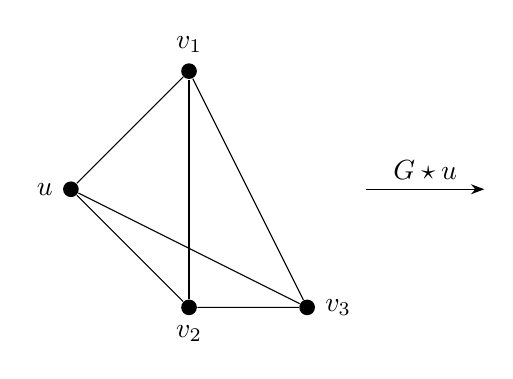
\begin{tikzpicture}[scale=1.5]
    % Define nodes
    \node[circle,fill,inner sep=2pt,label=left:$u$] (u) at (0,0) {};
    \node[circle,fill,inner sep=2pt,label=above:$v_1$] (v1) at (1,1) {};
    \node[circle,fill,inner sep=2pt,label=below:$v_2$] (v2) at (1,-1) {};
    \node[circle,fill,inner sep=2pt,label=right:$v_3$] (v3) at (2,-1) {};

    % Draw edges
    \draw (u) -- (v1);
    \draw (u) -- (v2);
    \draw (u) -- (v3);
    \draw (v1) -- (v2);
    \draw (v1) -- (v3);
    \draw (v2) -- (v3);

    % Arrow and label
    \draw[->,>=Stealth] (2.5,0) -- node[midway,above] {$G \star u$} (3.5,0);
\end{tikzpicture}

\begin{tikzpicture}[scale=1.5]
    % Define nodes
    \node[circle,fill,inner sep=2pt,label=left:$u$] (u) at (0,0) {};
    \node[circle,fill,inner sep=2pt,label=above:$v_1$] (v1) at (1,1) {};
    \node[circle,fill,inner sep=2pt,label=below:$v_2$] (v2) at (1,-1) {};
    \node[circle,fill,inner sep=2pt,label=right:$v_3$] (v3) at (2,-1) {};

    % Draw edges
    \draw (u) -- (v1);
    \draw (u) -- (v2);
    \draw (u) -- (v3);
    \draw[dashed] (v1) -- (v2);
    \draw[dashed] (v1) -- (v3);
    \draw[dashed] (v2) -- (v3);

    % Arrow and label
    \draw[->,>=Stealth] (2.5,0) -- node[midway,above] {} (3.5,0);
\end{tikzpicture}

\end{document}